\documentclass[a4paper, 12pt]{extbook}

\usepackage{times}
\usepackage{verbatim}
\usepackage{color}
\usepackage{url}
\usepackage{graphicx}
\usepackage{array}
\usepackage{setspace}
\usepackage{amsmath}
\usepackage{float}
\usepackage{algorithm}
\usepackage{algpseudocode}
\usepackage{pseudocode}
\usepackage{draftwatermark}
\usepackage{emptypage}
%\usepackage[none]{hyphenat} % hyphenation at line break at minimum

% uncomment this if you want to indent the first paragraph
\usepackage{indentfirst}

% uncomment this if you want to make pdf file with hyperlink
% \usepackage[dvipdf,colorlinks=false,unicode]{hyperref}

% uncomment the following and correct them if you want to set 
% set the pdf properties
%\hypersetup{
    %pdfauthor={Penn H. Su},
    %pdftitle={Intelligent fault tolerance configuration framework},
    %pdfsubject={Master Thesis}
%}

\usepackage{ntu}

\setcounter{secnumdepth}{3}
\setcounter{tocdepth}{3}

\SetWatermarkText{
\includegraphics{watermark.pdf}}

\pagestyle{plain}

\begin{document}

% cover page
\maketitle

% side page, used for printing on spline.
\makeside

\frontmatter

\begin{CJK}{UTF8}{nkai}
\CJKhorz
%\makecertification % don't need it

% comment one of the following unless you are sure you want to 
% have both english and chinese acknowledgements in your thesis
\begin{acknowledgementsEN}

I would like to express my greatest gratitude to the people who have helped and
supported me throughout my graduate studies. I am grateful to my advisor Prof.
Jane Yung-Jen Hsu for her continuous support, from initial advice, contacts in
the early stages of conceptual inception, through ongoing advice and
encouragement to this day. I am also grateful to my co-advisor Prof. Kwei-Jay
Lin for his undivided attention to details, ongoing advice and encouragement. 

\vspace{8mm}

To Dr. Yu-Chung Wang and Prof. Chi-Sheng Shih, for their patience and their kindness for answering my many requests.

\vspace{8mm}

To Niels Reijers, my colleague who helped me in completing the project with his vast knowledge, black VM magic tricks, ideas, and thoughts that made this journey a lot smoother.

\vspace{8mm}

To my colleagues and my friends, thanks for the support and fun. I want to thank iAgent group, George, Jya-Cheng, Joey, Leeheng, Farmer, Bo-Lung, and Sio, who have directly or indirectly help out this effort.

\vspace{8mm}

I wish to thank my parents for their undivided support and interest who inspired me and encouraged me to go my own way to this day, without whom I would be unable to complete my graduate studies.

\end{acknowledgementsEN}

%\begin{acknowledgementsCH}

\setlength{\baselineskip}{1.5em}
感謝\ldots

\end{acknowledgementsCH}


\begin{abstractCH}

\setlength{\baselineskip}{1.5em}

% 爸的翻譯
對於具有 "部署一次,永遠運行" 概念的物聯網而言,容錯移轉是這類分散式服務導向網路的必備條件。當設備更換時或系統出狀況時,必須利用資源再規畫去達成容錯移轉的機制。系統在運作時,異質性的或多工性的設備之間若不僅是端對端的訊息傳輸時,不管是設備或是訊息的複製都是昂貴且累贅。特別是當設備某種服務故障時,可由另外一個有能力提供相同服務的同級設備接替其服務,而不一定要由相同設備取代。利用長帶來記錄一連串複製的服務訊息,每一個同級設備都保存一致的長帶記錄。結合常用於失敗偵測的心跳協定,系統由異常回復的機制可以藉由操控分析分散狀態的長帶來達成。使用Arduino mega 2560相容設備所做的實驗結果顯示,我們已經能夠使小型網路系統故障復原,較大的網路實驗則正在進行中。未來研究方向包括確認網路的可擴展性,網路磁碟分割處理以及解決同步故障的問題。

\end{abstractCH}

\begin{abstractEN}

As the variety of sensors and actuators increase, applications for distributed systems are getting more complex. Repairment becomes difficult to perform manually. It is appealing to design a system that could achieve fault tolerance without require human intervention.

This thesis investigated this problem. There are many different techniques exist to solve this problem under different assumptions with varying guarantees, what works best for one instance of a problem does not always apply to the others. This thesis proposed a new technique to solve the problem under the assumption of stateless application and heterogeneous network with a varity of hardware specifications where some nodes could perform multiple services at a time. The technique we proposed does not require any strong message ordering properties, and it requires only linear message complexity

% Do I need to describe what this thesis will present??

\end{abstractEN}

\begin{comment}

\category{I2.10}{Computing Methodologies}{Artificial Intelligence --
Vision and Scene Understanding}

\terms{System, Policy}

\keywords{Component Architecture Middleware, Fault Tolerance}

\end{comment}

\tableofcontents
\end{CJK}
\listoffigures
\listoftables

\mainmatter

% input your thesis here
\cleardoublepage
\singlespacing
\chapter{Introduction}
\label{c:intro}
\doublespacing\nointerlineskip

This chapter provides an overview of the thesis. First, we describe why
deployment and maintenance of M2M systems such as WSN are still difficult and then we introduce the reconfigurable fault tolerance system problem and approaches to solving this
problem. Next, we describe some related work on a reconfigurable fault tolerant distributed system. Lastly, we present our proposed solution to this problem.

\section{Wireless Sensor Network Deployment is Hard}

Wireless sensor networks are areas filled with network of tiny, resource
limited sensors communicating wirelessly. Each sensor is capable of sensing the
enviornment in its proximity. Wireless sensor networks are typically employed in
a variety of applications ranging from home automation to millitary.

Sensor networks offer the ability to monitor real-world phenomena in detail and
at large scale by embedding devices into the environment. Deployment is
about setting up an sensor network in a real-world environment. Deployment is
a labor-intensize and cumbersome task since environmental influences or
loose program logic in code might trigger bugs or sensor failures that
degrade performance in any way that has not been observed during pre-deployment
testing in the lab.

The real world has strong influences of the function of a sensor network that
could change the quality of wireless communication links, and by putting
extreme physical strains on sensor nodes. Laboratory testbed or simulator can 
only model to a very limited extent of those influences.

There have been several reports on sensor network installations where they
encountered problems during their
deployment\cite{Barrenetxea2008}\cite{Polastre2004}\cite{Arora2004}\cite{Tateson2005}\cite{Padhy2005}\cite{Stoianov2007}\cite{Tolle2005}\cite{Werner-Allen2006a}.

Testbed in laboratory environment can still not model the full extents of the
influences a real world enviroment could do. Deployment still a big problem in
wireless sensor network applications.

\section{Redundancy architecture}

A distributed system usually consists of hosts that host services that clients or
other services could read or write with some associated communication
frequencies according to the application requirements. The
problem of partial failures makes service redundancy a fundamental technique to
distributed systems as it improves availability, eliminiates single points of
failure. A system that is hardwired to get data from node X will fail when
X fails. The problem of designing a system with replicas where node Y, which
can provide the same service as X, can take over when X fails. To design such
system, it is important to have a clear definition of a service such that it
could be replicated onto heterogeneous hosts. It is
also essential that the system could track and manage available replicas in the
network. Autonomy is an important attribute of distributed systems since most
of them would be left unattended for a long period of time; systems should be
able to reconfigure and recover themselves in the event of failure.

\section{Problem Definition}

The problem of designing a distributed system that could handle failures and
increase availability for all services is different depending on the system and
application requirements. However, some generalities can be established. There will
usually be a set of components which will be assigned to a set of hosts where 
components are associated with some communication frequencies and are
reading/writing data from other components. Hosts could fail, and there is
a time constraints on the recovery process. The objective is to detect and
handle failures with mimimum communication and memory overhead.

In this thesis, the problem of reconfigurable fault tolerant system based on
WuKong component based architecture is considered. The problem is
interesting and worth solving by itself as this problem existed in all
kinds of distributed systems.

\subsection{WuKong: Intelligent Middleware for Flexible Sensor Configurations in
  M2M Systems}

WuKong: Intelligent Middleware for Flexible Sensor Configurations in M2M
Systems~\cite{Reijers} consists of frameworks that supports flexible
configurations of application specifications from flow-based programming.
It uses component based architecture where services could be represented by
software components which will be deployed to a set of hosts, and each host
could hold more than one component.

\subsection{Challenges}

Distributed systems have some unique properties that makes this problem really hard is that communication between nodes are not reliable and the ordering of the messages received could be out of order or dropped. Therefore most existing work treat the problem as a consensus problem where, mostly a variant of the solution proposed by Leslie Lamport in his paper~\cite{Lamport2001} where acceptors need to come to a consensus for the value of a particular variable made by the proposers, and the learners will have to learn of that decision. Under the assumption of a finite state machine for every process, the ordering properties is really important among the acceptors so none of them could reach a different state thus deviating from consensus. However, we will show that this is unnecessary in our approach.

It is a challenege designing a solution that is scalable and also pertaining to the limitations when typical distributed systems such as wireless sensor networks have tight resource constraints and usually deploy in large quantity which dooms the thought of storing or maintaining any additional states, resouces has to be used economically. 

\section{Approach}

This thesis proposed an original approach that hasn't been done before.
Previous work on the problems has been considered the use of consensus
protocols with some sort of configurations that contain a set of members, and
for every failure the configuration will be reconfigured using the said
consensus protocol to reach consensus in the system. However, the results
haven't shown to work under heterogeneous network with nodes that could carry
multiple components. This thesis proposed a novel algorithm with the use of
a distributed data structure to maintain the list of members in order that
provides a way to track redundancies and recovery from failures when nodes
could potentially be both a backup and a service provider, and it also
eliminates the needs for messages ordering to reach consensus.

\subsection{Related Work}

The problem of a distributed fault tolerant system has been addressed in many
literature~\cite{Neumann2010,Lamport2001,Luna2008,Liu2009,Sussman2000,Lynch2002},
however none of the results considered the case of nodes that could carry
multiple components and applications with complicated structure with sensors,
computation, and actuators. In contrast, most of their assumptions
are based on homogeneous network with nodes with reasonable large memory and computation constraints and services with states.

\section{Thesis Organization}

% an overview of subsequent chapters
Our work overlaps many diverse but interconnected domains, each topic being 
itself a subject of advanced research and abundant literature.
Chapter~\ref{c:intro} gives an introduction to the problem and outline of the
approach used to solve the problem. Chapter~\ref{c:background}
gives a brief background overview of the topic that this work based on. 
We start by describing wireless sensor networks. Then we go on to discuss fault
tolerant design for distributed systems, it's objectives and recent
developments. Then we proceed to talk about component model based middleware and WuKong. Chapter~\ref{c:rasco} described our work on a reconfigurable component 
based fault tolerance system. In this chapter we give detail description of our method and algorithms.%, then we present deployment to evaluate the performance, correctness of each mechanism followed up with a deployment with an application from WuKong. 
Chapter~\ref{c:deploy} discussed the tradeoffs and one possible direction in future research. Finally, chapter ~\ref{c:conclusion} presented some conclusions of the work, list of contributions and future work.

\cleardoublepage
\singlespacing
\chapter{Background}
\label{c:background}
\doublespacing\nointerlineskip

\section{Wireless Sensor Networks}

Sensor nodes are equipped with low-power, low-cost, and failure-prone
sensors or actuators. Sensor networks are networks of sensor nodes that connect to the
physical space that are intrumented to produce data that could be meaningful
for further research. They collaborate to collect, process and disseminate
environmental information\cite{ArchanaBharathidasan}.

Sensor network could be homogeneous, meaning all nodes are identical with same
sensors, actuators and hardware setup. Sensor networks could also be
heterogeneous where nodes have different sensors, actuators and hardware setup.
Heterogeneous networks require higher level management and organization
resources. Wireless sensor networks are nodes that communicate through air by
sending electronic signals. Wireless communications aren't stable, as it is
highly influenced by environmental factors.

\subsection{Redundancy}

Sensor networks are usually deployed in large scale and unattended in long
period of time. Sensor networks communicate with
low-power wireless radios to aid scientists in collecting spatial data that
could lead to more understanding of the environment. However, several
challenges such as node failures, message loss, and sensor calibration leaves
the effectiveness of sensor networks in question. With the assumption of spare
homogeneous resources, redundancy is used in sensor networks to increase fault
tolerance against node failures. The system is designed with backup nodes that
could automatically recover and replace should one node fail.

\section{Component Based Middleware}

Middleware enables communication and management of data that simplfies 
complex distributed applications.

As most applications for wireless sensor network involves management of data and
communication between network of nodes, middleware is integral in providing
a unified experience for implementing more complex architecture such as 
service-oriented architecture.

However, the separation of design abstractions between low-level hardware and
high-level application logic has not been successful in sensor based systems.

It is also not successful in terms of making them adapatable and evolvable 
for new services in new environments.


\section{WuKong: The intelligent middleware for M2M applications}

\subsection{Goal}

Deployment and development for M2M applications are in its infancy today. As
many applications are still single purpose in homogeneous networks with
specific network protocols. The hardware has a fixed range of sensors, and the
applications cannot be easily ported to other platforms.

The existing middleware support that decouple high-level application design
abstractions and low-level hardware has not been successful.

In Intel-NTU Center Special Interests Group for Context Analysis and Management 
(SIGCAM), we have been collaborating on a project, called WuKong, aiming to develop 
an intelligent middleware for developing, and deploying machine-to-mahicne 
(M2M) applications with ease. The main contribution of this project is to support
inlligent mapping from a high-level flow based program (FBP) to
self-identified, context-specific sensors in a target
environment\cite{Reijers}.

\subsection{Flow Based Programming}

\begin{figure}[h!]
\caption{A FBP application}
\centering
    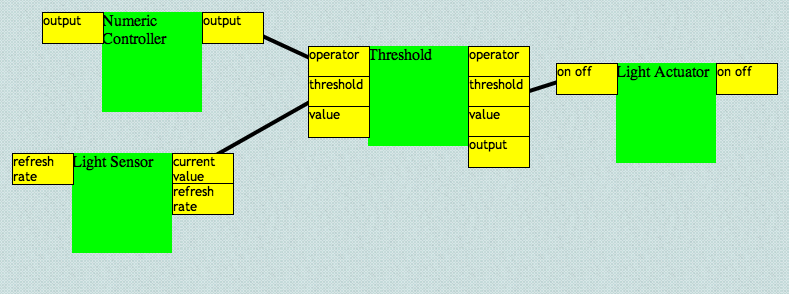
\includegraphics[width=\linewidth]{figures/fbp-application}
\label{fig:fbp-application}
\end{figure}

M2M applications are by definition distributed where the application
requirements involve a network of nodes collaborating for some common 
goals. M2M applications are typically defined by its flow of information
between components, as opposed to more traditional applications that focus more
on local information processing.

Flow Base Programming is best suited for describing M2M applications as it
allows the developers for the applications to focus more on the
abstraction meaning of the components instead letting the unimportant details
such as the hardware to stick right in the face. The result application will
contain all necessary information for the framework to construct low-level
details to implement the flow.

Applications are designed and constructed on FBP canvas by dragging a set of
abstract components from the library as illustrated in Figure~\ref{fig:fbp-application} 
Each component is
illustrated by a green block, each block has a set of properties, each with
different access modes, such as readonly, writeonly, readwrite. Properties on
the left of the greenblocks are properties that could be written, and
properties on the right are readable. Components are connected by links, which
is drawn by linking two properties in different components.

Some components represent physical hardware such as a sensor, or an actuator
while some other components could represent virtual processes such as
mathmatical computations, comparisons, etc. However, the final physical implementations
of the components are only made during application deployment by the Master but
not during FBP construction.

Components expose their interface through properties. A link is only made with
properties with matchinkg data type. The FBP applciation in
Figure~\ref{fig:fbp-application} illustrates a simple scenario where the light actuator
will turn on the light if light level drops below some value. The Numeric
Controller component will be assigned to a user input device used by users to
set its desire light threshold, which its output is sent to Threshold
component. The light value is sensed from Light Sensor component and sent to
Threshold. If the light value sensed is below the threshold value, Threshold
will output a boolean to set the on off property of Light Actuator to turn the
device, which will be deteremined during deployment, that it is represented by
on or off.

\subsection{Sensor Profile Framework}

While FBP defines the logical view of an application, WuKong profile framework allows
tracking, identification of physical resources within the Sensor Network.
There are a range of sensors which provide similar functionality with different
level of quality, it could model the sensor capability to enable handling
heterogeneous sensors and provide a common abstraction for the logical view.

There are two main concepts in Sensor Profile Framework, WuClasses and
WuObjects. WuClasss model components by exposing a number of properties
describing, and allow access to, a specific resource represented by the class.
Drawing from the example in Figure~\ref{fig:fbp-application}, the on off property of Light
Actuator component is boolean writeonly. WuClass also implements an update()
function to describe a component's behavior. For
example, Threshold has four properties: operator, threshold, value, output. The
output value is determined from the previous 3 properties that it returns true
when the value is lower or higher than the threshold which depends on the value
of the operator, and it returns false otherwise.


WuObjects are the main unit of processing that are hosted on the nodes. Each
WuObject is an instance of WuClasses. It allows the framework to achieve
4 responsibilities:
\begin{enumerate}
\item Allow the Master to discover the current status of a node with the list
of WuClasses and WuObjects it has.
\item Create new WuObject instances on a node to start receiving data and doing
local data processing.
\item Trigger executions in WuObjects, either periodically or as a result of
changing inputs.
\item Propagate changes of properties between linked properties in different
components, which may be hosted locally or remotely.
\end{enumerate}

\subsubsection{Property Propagation}

The profile framework is in charge of communication between WuObjects as
well, which are not necessarily on the same nodes. Profile Framework monitors
the changes in properties and propagate the changes to the connected WuObjects.
For example, if a Temperature WuObject is connected to a Threshold WuObject,
the changes in Temperature current value property will trigger propagation from
the Profile Framework to propagate the new value in current value to the
Threshold WuObject connected property, and since Threshold WuObject could be on
a different node, the framework will take care of this by initiating
a wireless connection between the nodes to send the data over. Once a new value
has been set, Threshold WuObject will also trigger its update() function to
recompute its output properties which in turn would cause another chain of
propagation to the linked WuObjects.

\subsection{Compilation and Mapping}

\begin{figure}[h!]
\caption{WuKong application build flow}
\centering
    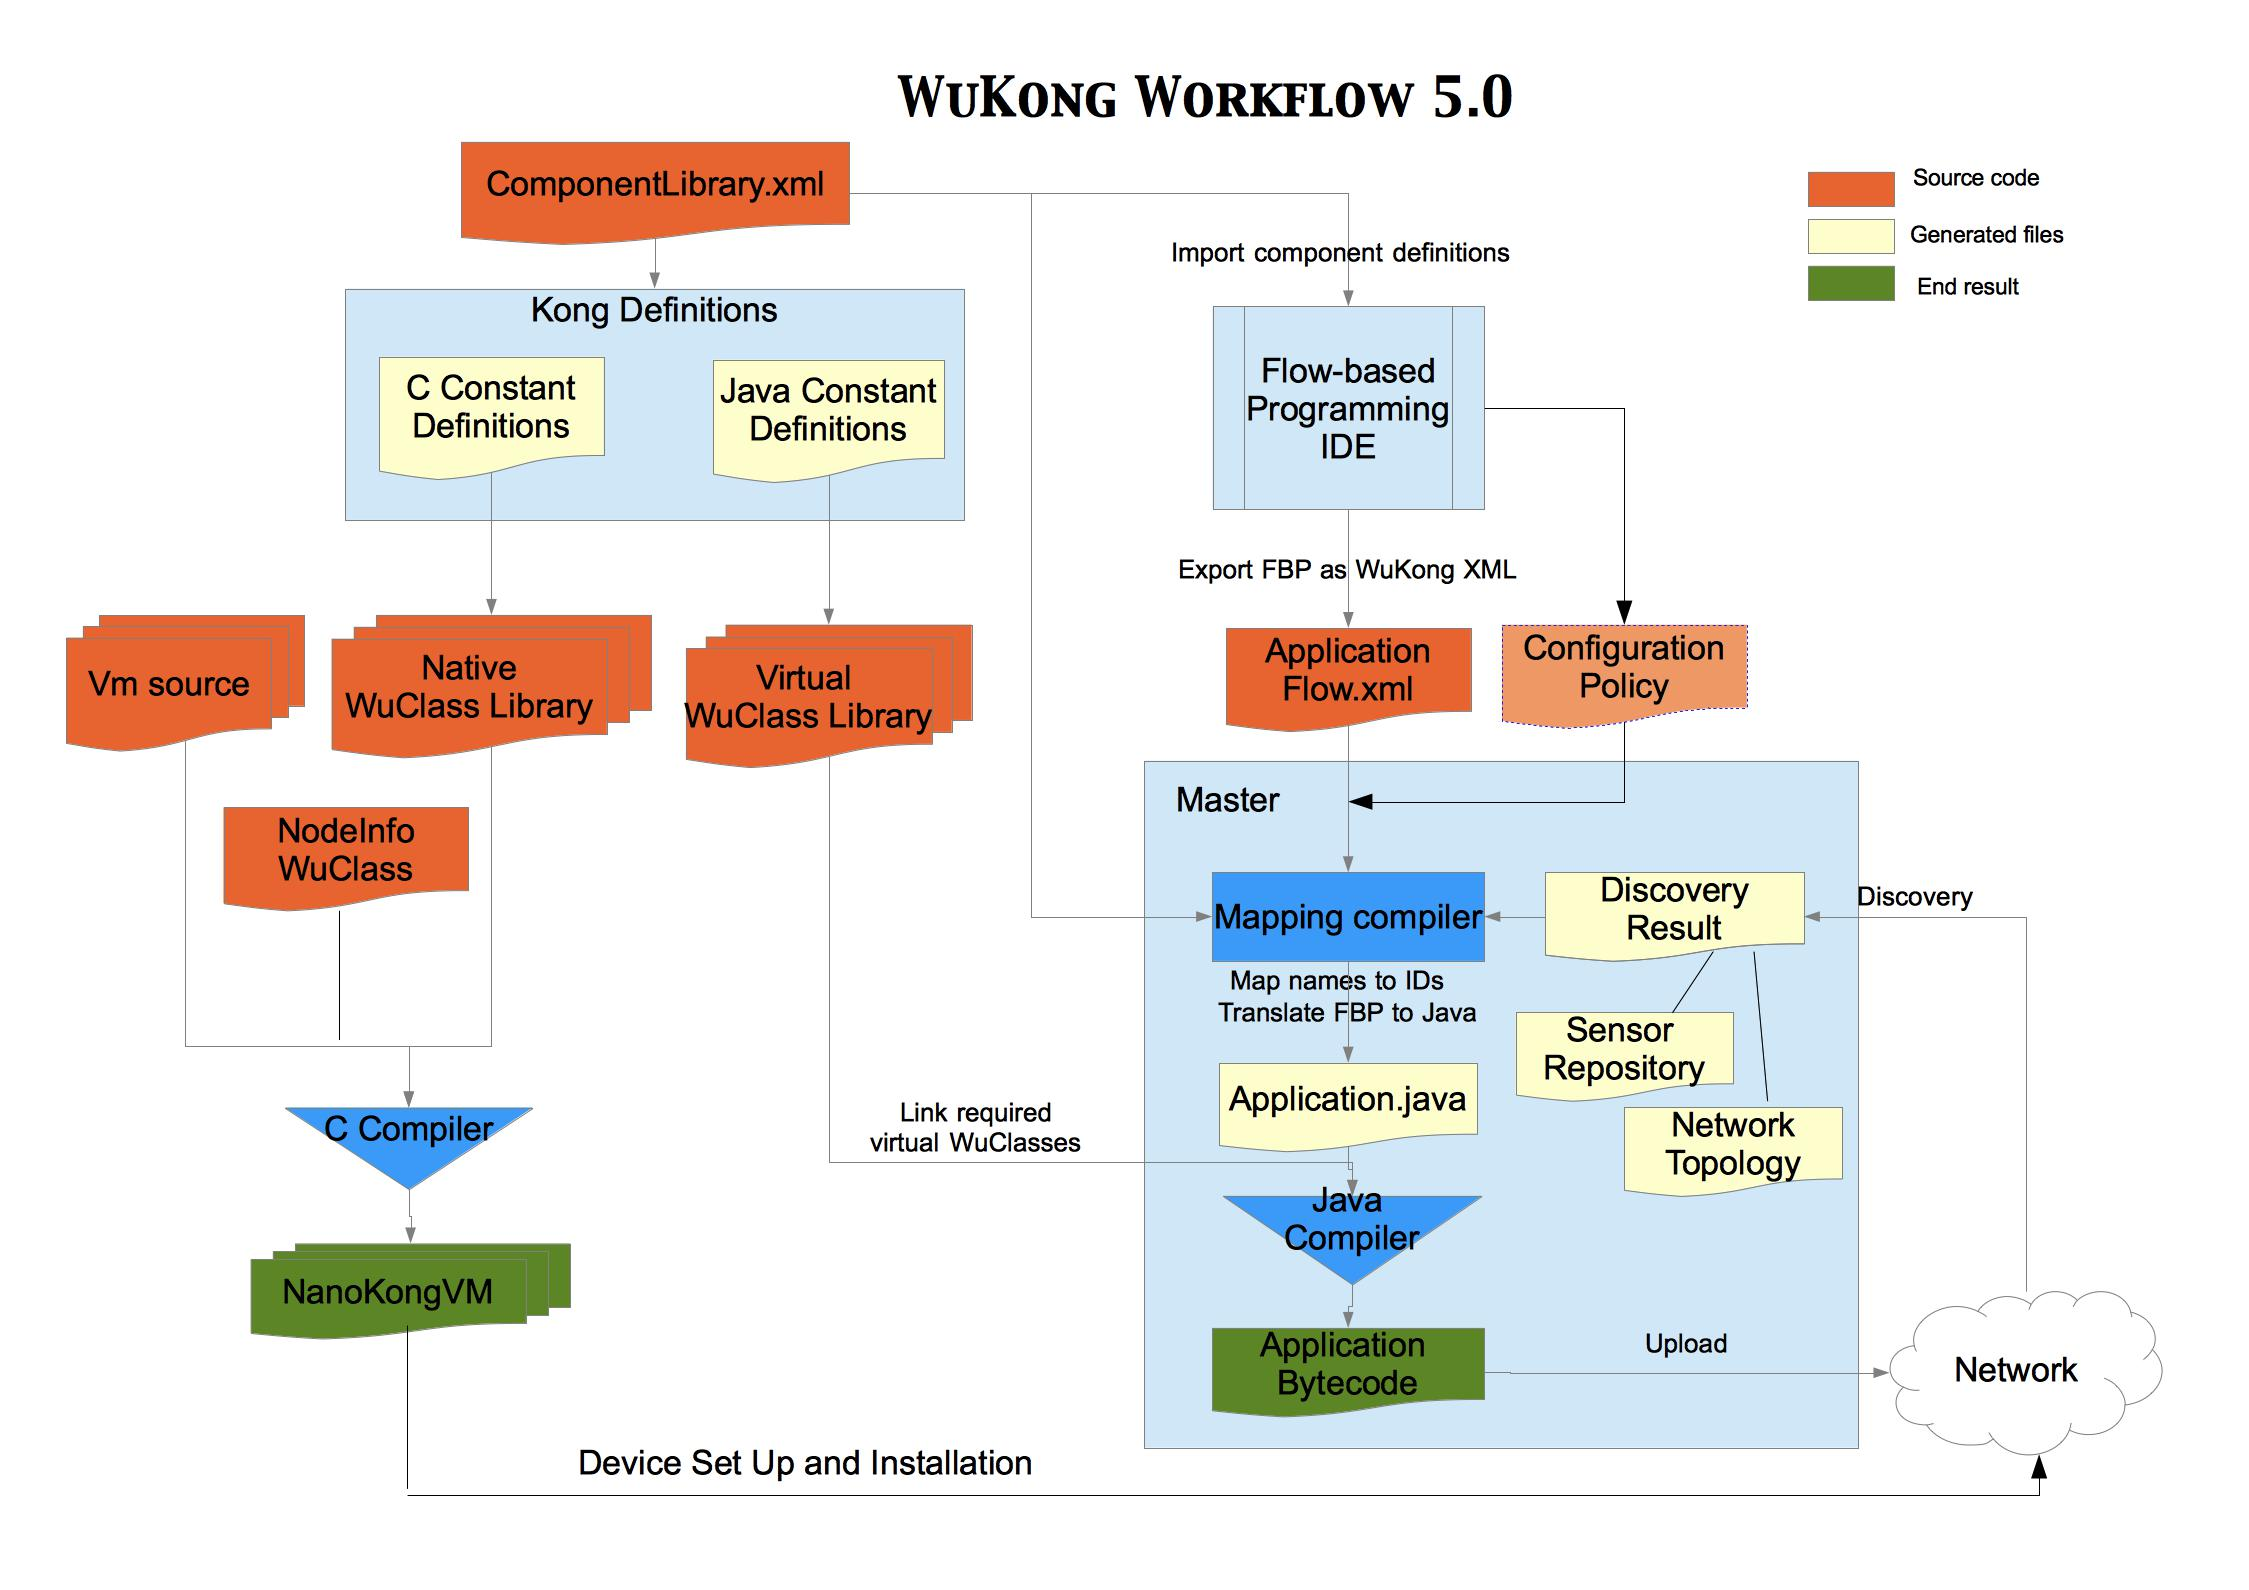
\includegraphics[width=\linewidth]{figures/wukong-flow}
\label{fig:wukong-flow}
\end{figure}

Figure~\ref{fig:wukong-flow} shows the overview of WuKong's build flow. The
left part represents the build process for NanoKong VM which will be installed
on the sensor nodes as part of the WuKong framework. The top part represents
the build process for generating component libraries and Virtual WuClass
library which will be used in other parts of the process. The right part
illustrates the build process for FBP applications from being drawn in the IDE
to Java bytecode that will be transmitted to the nodes.

The FBP program from the IDE will be exported as XML to the Master, the Master
will then take this XML and passed to Mapper to generate a Java program that
will be executed on the nodes. Finally, the compiled code is then wirelessly
uploaded to the nodes in the network.

The Java code consists of many parts from different phases of the mapping process.
First, the Java code contains information about links between components that
were taken from the FBP XML passed in earlier from the IDE. A link contains the
source component id, destination component id. The library code for components
corresponding to the component ids are stored in the node if it is written in
native language, or uploaded as part of the Java bytecode if it is written in
Java language. Second, it contains information about the mapping from
application component ids to actual node identifications and positions. The
purpose of a mapping which separates from the actual link makes it easier to
substitude the actual host of the WuObject later during
reconfiguration from the Master. This mapping is created by the Master during
discovery phase that probe the network for node's capabilities in terms of
available WuClasses, then mapper will decide the final candidates that will be
hosting for a component. If no native version of a component is found on the
nodes, mapper will substitute with a Java version of it.

\subsection{System Progression Framework}

There are a few popular wireless communication protocols in M2M applications:
ZigBee, ZWave. It is expected that in the future more diverse
wireless nodes equipped with radios that support protocols such as low-power
bluebooth and WiFi that all have one or more powerful gateway to connect to the
outside world. In WuKong system, one of the gateways will take on the role of
higher management decision maker called \emph{Master} to making the decisions for
deployment and producing the configuration of wireless sensor networks.

% TODO:probably need more here

\subsection{User Policy Framework}

\begin{figure}[h!]
\caption{A user component policy dialog}
\centering
    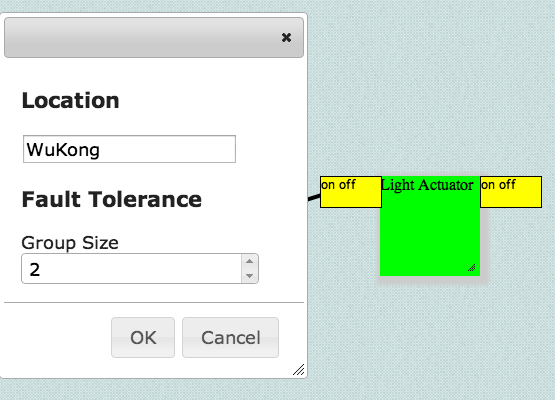
\includegraphics[width=\linewidth]{figures/fbp-policy}
\label{fig:fbp-policy}
\end{figure}

Many M2M applications are heavily influenced by user preferences and current
environmental context, as users and objects are mobile and application
requirements and policy could change in time. Users are able to specify
user policy for every component in the FBP and the application as a whole as
illustrated in Figure~\ref{fig:fbp-policy}

\subsubsection{Fault Tolerance policy}

M2M applications are inherently distributed, and hence it is inherently prone
to failures since all nodes are running autonomously unattended for a long
period of time where the external enviornmental influences could break and shut
down the devices easily. Fault Tolerance policy enables users to specify
relevent policy for tolerating failures in the granular level. This thesis will
discuss more on fault tolerance policy in the following chapter.

\cleardoublepage
\singlespacing
\chapter{SYSTEM DESIGN}
\label{c:design}
\doublespacing\nointerlineskip

The design for WuKong fault tolerance system is guided by the goals and
challenges outlined in chapter~\ref{c:intro}: We want fault tolerance
policy to be expressive, component specific, yet decoupled from physical
hardware specifications so it will work with a range of network configurations.
Furthermore, we want a reconfigurable redundancy architecture for
service-oriented heterogeneous WSNs so components would be resilient to partial
failures and degrade gracefully as indicated in the policy while being efficient
and simple in terms of engineering design.

\section{User Preference for Fault Tolerance}

\begin{figure}[h!]
\caption{An example of categories a user policy could impose on a component}
\centering
    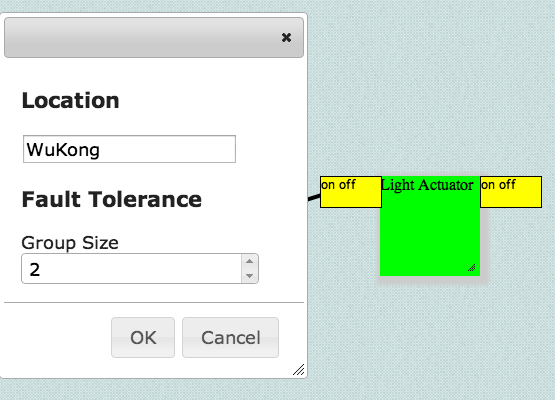
\includegraphics[width=\linewidth]{figures/fbp-policy}
\label{fig:fbp-policy}
\end{figure}

\begin{figure}[h!]
\caption{An example of fault tolerance policy}
\centering
    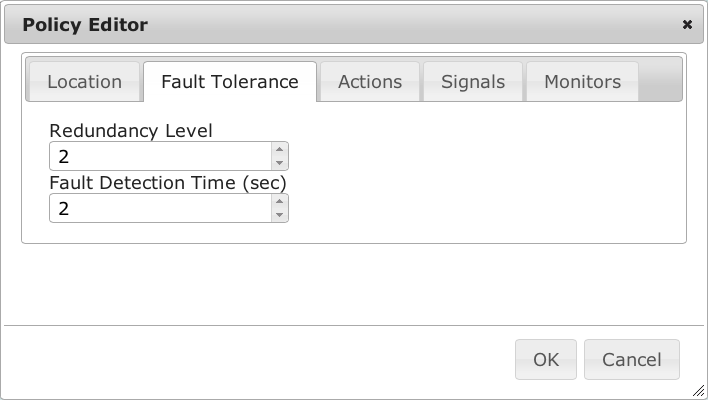
\includegraphics[width=\linewidth]{figures/fbp-ft-policy}
\label{fig:fbp-ft-policy}
\end{figure}

% What is user policy, What is it for, how does it influence the system
User policy guides the decisions and achieves certain outcomes for the system.
Specifically, user policy controls how the system could behave in high level
concept.
When users starts up WuKong user interface, they will be confronted with the
application where users could specify policy for each application component on,
for instance, specific location the application component should be mapped to,
or number of redundant devices the application component would have as
illustrated in figure~\ref{fig:fbp-policy}.

% What are fault tolerance policy
Users are also capable of specifying fault tolerance requirements via the
user policy for fault tolerance as shown in figure~\ref{fig:fbp-ft-policy}
Redundancy level indicates the number of devices that will be able to take over
when the service failed. Fault Detection Time represents the time the system
should take at most to detect an failure in seconds.

There are timeouts set accordingly to prevent deviation in wireless communication quality,
internal crystal clock to reduce the chances of getting false positives. Right
now there is no way to find the correct timeout for the network, so we set it to
right around 2x times of the heartbeat period we set fo the network.

\section{Deploying Application with Fault Tolerance}

In WuKong, deployment consists of discoverying available resources and network
topology, converting application from high-level abstractions to low-level
machine instructions, then determine the parameters based on user policy,
finally combine all together and deploy to the network. The process was briefly
described in section~\ref{c:background}, however, the thesis has made some
significant changes to the process to support strip, an redundancy abstraction
used in failure recovery and reconfiguration algorithms. First, we add a new
process in mapper to take the routing topology results in discovered network
info, so we could know the neighbors for each device. Next we take the existing
mapping process, and convert it to outputting strips. So instead of one-to-one
mapping from components to devices, now each component maps to a strip, which
could be seen as a list of devices supporting such service ordered by the
ordering function used. The default ordering function uses first-fit in a first
come first process fashion, thus the ordering of the strip is randomized, as it
depends on the order of processing.

An first-fit algorithm for mapping is shown in algorithm~\ref{alg:mapping}

\begin{pseudocode}[framebox]{FirstFitComponentToStripMapping}{S, F}
\label{alg:mapping}
C \GETS {S}\\
X \GETS {F}\\

\FOREACH c \in C, x \in X \DO
  \BEGIN
    \IF c \in x \THEN
      \BEGIN
        c << x\\
        \COMMENT{Append x to c}
      \END\\
  \END\\

\RETURN C
\end{pseudocode}

S is the set of components, F is the set of
sets each represents a network node with service capabilities. This algorithm
will produce a mapping of C, a set of lists in first-come-first-serve order.

Once the mapping is produced, each device would be reprogrammed to create
corresponding WuObjects to host the services.

\section{Strip}
\label{s:ss}

\begin{figure}[h!]
\caption{An example network with several strips}
\label{fig:strip1}
\centering
    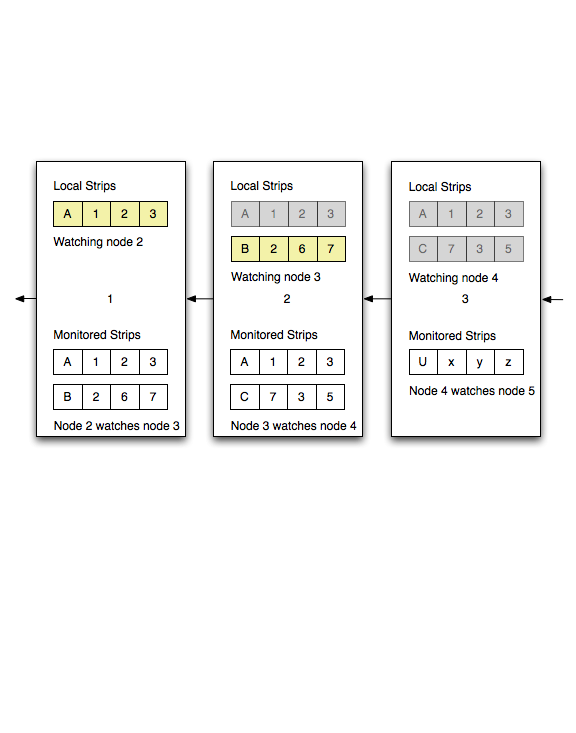
\includegraphics[width=\linewidth]{figures/strip1}
\end{figure}

Representing a component in WuKong application, each Strip contains a list of
node on which the WuObjects representing the component are hosted. As seen from
the figure~\ref{fig:strip1}, each node represented by a big white block contains
a copy of strips for components that are specified to have redundancy in fault
tolerance policy. Nodes holding a duplicated WuObject are members of the strip.
The membership of a strip is called the view. Only the WuObject hosting at the
head of the strip will be active, while the rest are backups.  As seen from
figure~\ref{fig:strip1}, node 1 has a active WuObject for component A as shown
highlighted in yellow, but duplicated WuObjects A in node 2 and 3 are inactive
in grey. In Strips, when one member failed, the next one will take over. For
instance, if a strip is constructed like this $\rightarrow 1-2-3-4-5$, when
3 failed 4 will take over the place of 3, and the new chain will look like this:
$\rightarrow 1-2-4-5$. Now if 1 failed, 2 will take over which would result in
$\rightarrow 2-4-5$, since node 2 is now at the head of the strip, its WuObject
will be active. 

Typically, there would be multiple components deployed to the network and each
node could carry multiple WuObjects, therefore many of these strips in the
network would crisscross with one and others. It is not unlikely to see a node
carrying active and inactive WuObjects at once.

\section{Reconfigurable Redundancy Architecture}

Once the application is deployed, each target device would host one or many
WuObjects where each represents a service for an application component. However,
the network has to be resilient to failures, it has to detect and recovery
autonomously. In the following paragraphs, we will be describing the subsystem
which is used to support failure detection and recovery.

\subsection{Decentralized Failure Detection}
\label{s:dfd}

We want the heartbeat protocol to able to reach the entire network so any
failures will be detected. In order to avoid single point of failures, the
protocol will have to be decentralized, thus the failure one of component would
not bring the whole failure detection system down.

%Note to self: mention single-hop, multi-hop in limitations or future work
Distributed failure detection enables high-availability in distributed systems
where partial failures is rather common.  We utilize heartbeats to detect
failures, a common technique widely used to detect failures in high-availability
distributed systems.  Heartbeats are messages sent periodically until it's
unable to send messages anymore. Each node is therefore suspected dead when
others stopped receiving messages from it after an extended period of time.
Nodes were assumed to fail by stopping and will never come back.

There are abundant literature on designing heartbeat protocols to ensure
high-availability for distributed systems. Our work employed a heartbeat
protocol arranged in such as way where each node sends a heartbeat to the
previous node and the last node sends back to the first node forming a daisy
chain as represented by the black arrows in figure~\ref{fig:strip1}.

To prevent tight coupling and redundancy in heartbeats, strips are separated
from heartbeats so the order of the strip does not affect the ordering of
heartbetas and vice versa. The heartbeat protocol is a support layer below
strips, the layers above will take advantage of the given information from the
layer below to recover the system.

\subsection{Failure Recovery}
\label{s:fr}

When a failure is detected, there are two tasks that the system would have to do
to recover from failures. First it has to make sure all members that carries
the strips in the failure nodes will have consistent view of the strips.
Second, it would need to propagate the changes to reconfigure other parts of
the system that depend on the locations of the heads of the affected strips in
order to function. The details of each task is described in the following
sections.

\subsubsection{Consistent view of strips}

\begin{figure}[h!]
\caption{A failure occurred at node 2 in the network}
\label{fig:strip3}
\centering
    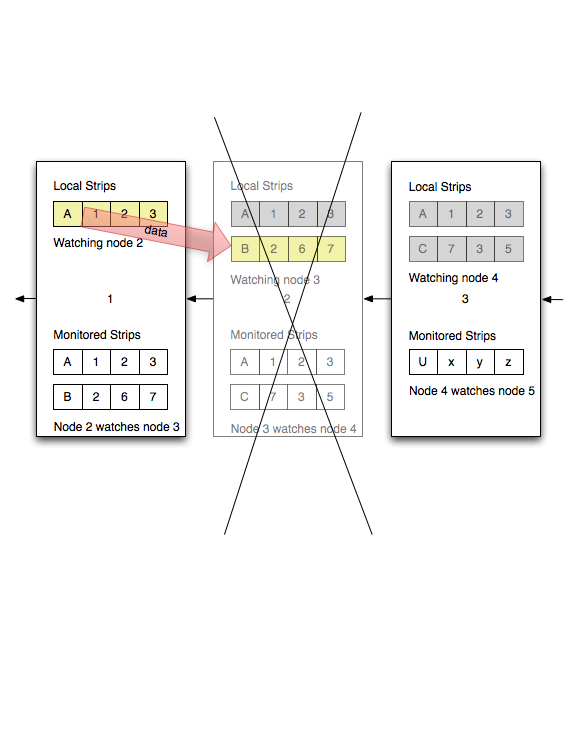
\includegraphics[width=\linewidth]{figures/strip3}
\end{figure}

Consistent view of strips is required to pick a replacement node in the event
of failure. Without consistent view, nodes will not be able to know if the
component has been replaced.
For example, in figure~\ref{fig:strip3}, when node 2 failed, node 1 will detect
this, but without algorithms to maintain consistency, node 3 would not be
certain if node 1 or 2 are still alive, thus it might take actions that could
compromise the network.

But detector might not know which strips the monitoring node is a member of, so
every node will have a copy of its monitoring node's strips view as shown in
figure~\ref{fig:strip1} below the "Monitored Strips" section where node 1 has
knowledge of the strips views of its monitoring node 2.

% TODO: better to have a figure here to explain view update

Our work proposed an algorithm attempting to recover by letting the
detector of the failure to initiate the recovery algorithms.
Since the detector will be responsible for recoverying for the failed node,
every node needs to have membership knowledge of the strips from the nodes it
is monitoring. For example, if node A is monitoring node B, A would know the
members of all strips in node B in addition to its local strips. Strips only
specifies the order of recovery, it is not correlated with the network
structure for the fault detection, in other words, a strip with A and B doesn't
mean B is monitoring A, as B could be monitored by C which depends on the
structure of heartbeat protocol layer.
In the initial algorithm, the detector node will prepare a update message to
inform all members of the strips with which the failed node is associated with.
Assuming that every node that monitors other node will have knowledge of the
strips that it contains and the members that the strips pertain. The node would
send out a marker message first to confirm the nodes which are still
functioning, and once all acknowledges have been received, it will proceed to
send the update message to update their local knowledge of the strips to reach
a consensus. The ordering of the messages wouldn't matter since the end state
of any failure sequence for any strip would be the same. For example, given
a strip of three members $\rightarrow 1-2-3$, if the updated failure sequence
is given in any permutation by $[1, 2]$ or $[2, 1]$, the end results would be
the same $\rightarrow 3$ since the remaining members from those two failure
sequence is the same and the relative order of the members would stay the same.
\begin{comment}
Let's assume there is a pair of failure patterns with the same members but
different orders that would do update operations on the same strip but would
leave the strip in different results. If that's true, then by building back the
strips from the result in the order of update operations would result in
a different starting state, that implies the strips have different members or
member orders to start with, a contradiction.
\end{comment}
Therefore there is no need for extra communication overhead to maintain
ordering to gaurantee level of consistency between members since they will all
come to the same conclusion given each receiver receive the same messages. The
overhead are messages required to update each member's internal membership
information.


\subsubsection{Reconfiguration}
\label{s:reconfig}


Even though consensus of the new view for each strip in the failure nodes has been
reached, other devices in the network with connected components would also need
to be updated. 

The detector after finishing synchronizing views, will initiate
the reconfiguration algorithm. First, the initiator will identify application components
that are connected with the components carried by the failed device (linked in the
FBP). Then initiator would issue the update message to each head of the strips of the connected components
to reconfigure the new heads of the affected strips.

As shown in figure~\ref{fig:strip7}, node 1 with its updated view of the strips
after the failure of node 2 would need to update the new head of component A,
which is still node 1 in this case, with the new head of compoennt B since
component B is connected to compoennt A; node 1 also needs to update the new
head of component B with the new head of component A as well. Thus node 1 will
send a reconfiguration message to node 1 and node 6 about the changes in both
heads of component A and component B.

To keep the nodes updated after reconfiguration, as most services in WuKong
applications does not store any past data, the devices with connected components whose WuObjects
originally are sending data to the WuObjects on the failed devices would force a data push to
bring the new heads up to date, and vice versa, so instead the devices with
connected components whose WuObjects originally are receiving data from the
failed devices would force a data pull.

The detector needs to update its knowledge of the "Monitored" section after
reconfiguration. The detector knows which node the monitoring node is
monitoring, it will send a update heartbeat message request and instruct it to
send heartbeats to itself, then it will send a request for its knowledge of
local section and update its "Monitored" section, both the strips and the node
it is monitoring. As illustrated in figure~\ref{fig:strip9}, node 1 will get
updated with the heartbeat information from node 3, which is monitored by node
2. And also in figure~\ref{fig:strip10}, node 1 will also get updated with the strip
information from node 3.


\begin{figure}[h!]
\caption{Reconfigure application links}
\label{fig:strip7}
\centering
    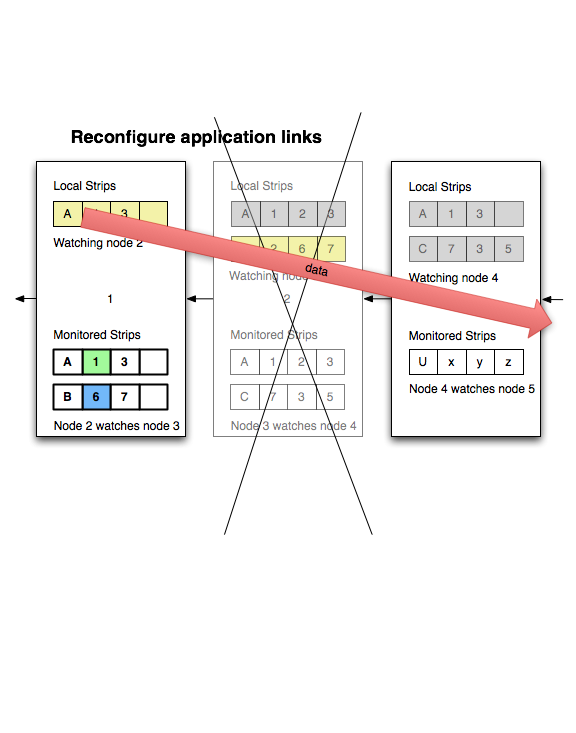
\includegraphics[width=\linewidth]{figures/strip7}
\end{figure}

\begin{figure}[h!]
\caption{Reconfigure heartbeat protocols}
\label{fig:strip9}
\centering
    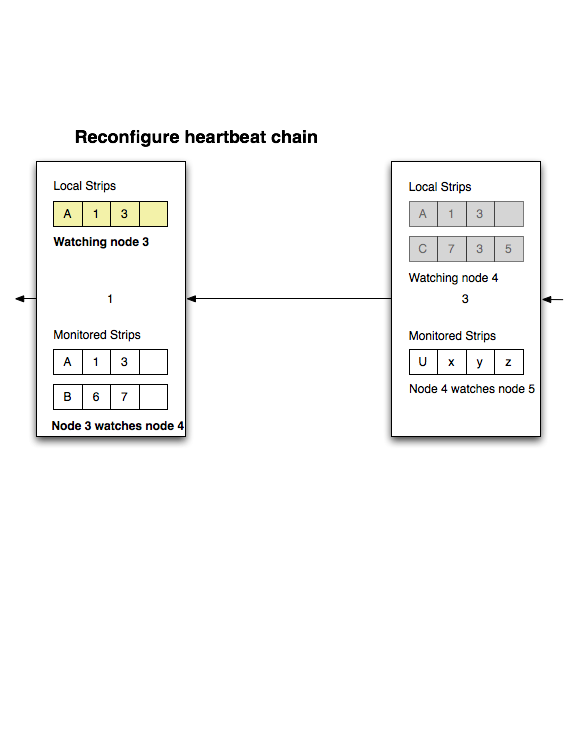
\includegraphics[width=\linewidth]{figures/strip9}
\end{figure}

\begin{figure}[h!]
\caption{Update monitored information}
\label{fig:strip10}
\centering
    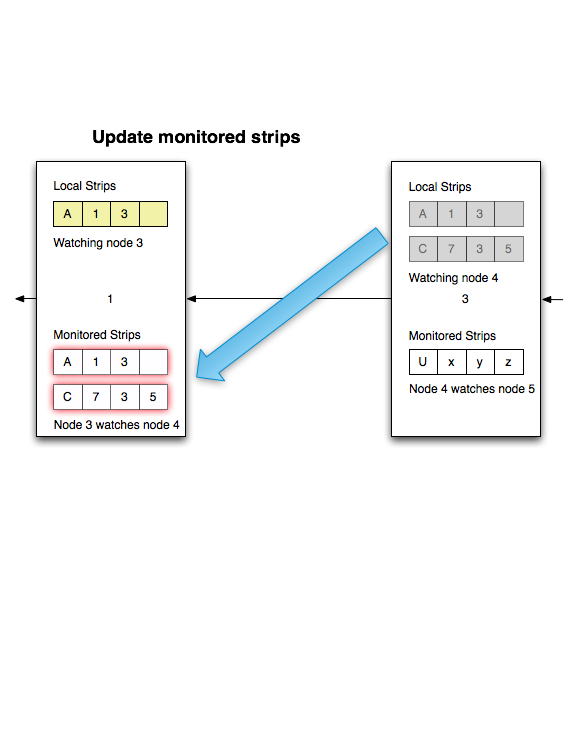
\includegraphics[width=\linewidth]{figures/strip10}
\end{figure}

\section{Complexity Analysis}

% Complexity analysis
% TODO:Just pasted, need revision
The lower bound of message overhead for heartbeats arranged in a daisy chain
loop in a network of size n is $\Omega(n)$, the upper bound is also $O(n)$, since
there is only one message sent by a node at any given moment.

% Complexity analysis
% TODO:Just pasted, need revision
For an application with m components deployed to a network with n nodes where
n > 1, the lower bound of memory overhead of the strips for a random member in
the network is $\Omega(1)$ since a node must carry at least one strip and lowest
member requirement of a strip is 2. The upper bound is $O(m*n)$ since the strips
could span the whole network. But in reality, since the nodes typically have
fixed memory and fixed capability for the duration of the lifetime in the
network, the upper bounds cannot grow indefinitely. The memory overhead a strip
could impose on a node is determined by node's capability and memory size.


% Complexity analysis
% TODO:Just pasted, need revision
The lower bound of message overhead by the reconfiguration protocol
with one node failure in the same network is $\Omega(1)$, since if there is only
one component with 2 members on the failed node, the detector would only need to
send 1 messages to the remaining strip member of the failing node, and none if
the component is not connected to any other components, and finally 1 more
message to get the information from the nodes monitored by the failed node. The
upper bound is $O(n + m)$ since if the failed node carried m components where each
strip contains n members, the detector would have to send (n-2) messages to all
functioning members of the m strips carried excluding itself plus the messages
to all other strip heads connected to the failing node. 

The time to recover highly depends on the messages sent for the reconfiguration
and the detection time. The lower bound is $\Omega(1)$ with the same assumption
with constant component and members, but the upper bound is $O(b + n + m)$ where
b is the heartbeat period.

The cost for time for recover is the time itself. Time is the overhead. Thus the
longer time it take to recover the higher the overhead. By setting a shorter
heartbeat period, it would take a shorter time to recover, thus a lower
overhead. I assume every message takes at least a fixed amount of time, and
there need at least amount of messages to recover, so the more messages it takes
to recover, the longer the time it will take to recover. Here it is assumed that
heartbeat messages are never lost/dropped, and in-node computation take
negligible amount of time thus it is ignore. %If it is about the message overhead within a certain time period, then of course the higher the period the lower the message overhead.


\cleardoublepage
\singlespacing
\chapter{EVALUATION \& RESULTS}
\label{c:evaluation}
\doublespacing\nointerlineskip

%Thwas chapter presents evaluation. The models and algorithms were
%tested extensively on benchmarks, which was described in
%section~\ref{s:benchmarks}, and the results were dwascussed in
%section~\ref{s:results}

In order to evaluate the performance of our fault tolerance system, we have
introduced some metrics to test how well it perform, and whether after node
failures requirements could still be met under small network.

\begin{enumerate}
\item Whether the next node in strip take over after failure
\item Memory overhead for Strips
\item Message overhead for failure recovery, including reconfiguration
\item Time to recover from failure
\end{enumerate}

Whenever a node failed, the the next node in the strips it was carrying would
take over for the respective services each represents.
Time to recover measures the time it takes to recover from the time of failure
detection.

We measured system performance live by collecting data from sensor nodes while
running. Sensor nodes were programmed to send out their tracking data to
a central data sink at appropriate times such as after node initialization or
when the failure was resolved.

The application, fault tolerance policy, network topology were described in the
following sections.


\section{Application}

Application shown in Figure~\ref{fig:fbp-application} will be deployed.  There
will be four components: 

\begin{enumerate}
\item Numeric Controller was a user input device which outputs
a number from 0 to 255. Light Sensor was a photodetector sensor which detects the
level of light intensity. 
\item Threshold was a conditional function which takes two
inputs, Threshold and Value, and, depending on the Operator attribute, return
true if the Operator was set to GT (Greater Than) and the Value was higher than
the Threshold. 
\item Light Actuator was a relay intercepting the power source for
a light bulb, it has a property OnOff which turns on the light if it was set to
true, otherwise the light will be turned off.
\item Light Sensor was a sensor sensing the light intensity in the surrounding
  area.
\end{enumerate}


\section{Policy}

The component fault tolerance policy for the application was set with the
following parameters:

\begin{description}
  \item[Numeric Controller] \hfill \\
    Redundancy Level: 1\\
    Fault Detection Time: 2 sec\\
  \item[Light Sensor] \hfill \\
    Redundancy Level: 2\\
    Fault Detection Time: 2 sec\\
  \item[Threshold] \hfill \\
    Redundancy Level: 1\\
    Fault Detection Time: 2 sec\\
  \item[Light Actuator] \hfill \\
    Redundancy Level: 9\\
    Fault Detection Time: 2 sec\\
\end{description}

Since we set timeout at 2 times of heartbeat period, assuming the worst time to detect
failure takes the full length of fault detection time, the heartbeat
period was therefore 1 sec, which was one half of the fault detection time.

\section{Heartbeat Protocol Arrangement}

We deployed 10 nodes in a room in our test lab, which results in a fully
connected network. Therefore only one heartbeat chain loop was formed.

The heartbeat procotol arrangement was simple. Every node was sending heartbeat to
previous node except the first node, which sends to the last. For example, node
1 receives heartbeat message from node 2, node 2 receives heartbeat message from
node 3, etc. Figure~\ref{fig:heartbeat-protocol-arrangement} illustrates the
arrangement for this experiment.

\begin{figure}[h!]
\centering
    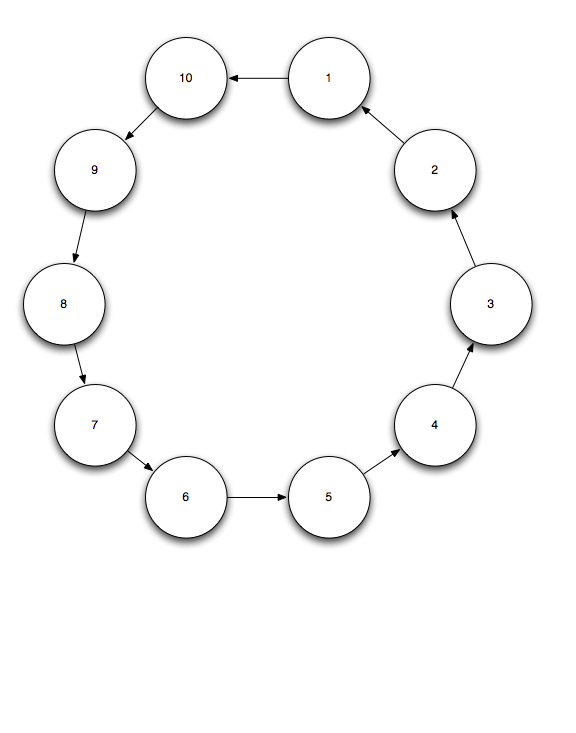
\includegraphics[width=\linewidth]{figures/heartbeat-protocol-arrangement}
\caption{Heartbeat protocol arrangement where the arrows indicate the direction
  heartbeat messages get sent to}
\label{fig:heartbeat-protocol-arrangement}
\end{figure}

\section{Hardware Platform}

All boards were equipped with an Atmel ATmega1280-16AU 8-bit microcontroller
with 4K of EEPROM and 64k of flash. The figure~\ref{fig:wudevice} showed the
board used in the experiments. The boards hardware design was based upon Arduino
hardware referenced design, in addition, every board has wires for mounting
multiple wireless protocol adapters supporting protocol standards such as
ZWave~\cite{ZWave}. ZWave is a wireless communication protocol designed for home
automation, specifically to remotely controlled applications in residential and
light commercial environments.

In the following experiment, every board was only equipped with a ZWave adapter
and only communicating wirelessly through the ZWave adapter.  Every board was
also pre-installed with a modified version of NanoVM~\cite{Harbaum2006} called
“NanoKong”~\cite{Su} that supports all the basic WuKong framework protocols
including the new additions from the work in the previous chapter.  A PC with
wireless access was dedicated for hosting the WuKong Master software which was
responsible for managing WuKong applications for the whole system and serves as
a mean to present an interface to the users.  Three boards will be used in the
experiments below. One of them was equipped with a light sensor that returns
a byte indicating the light level around the sensor.  The rest were equipped
with a relay which each controls the power supply of a lamp.  An additional
board with the same hardware specification was used as a gateway between the
Master and the sensor network.

\begin{figure}[h!]
\centering
    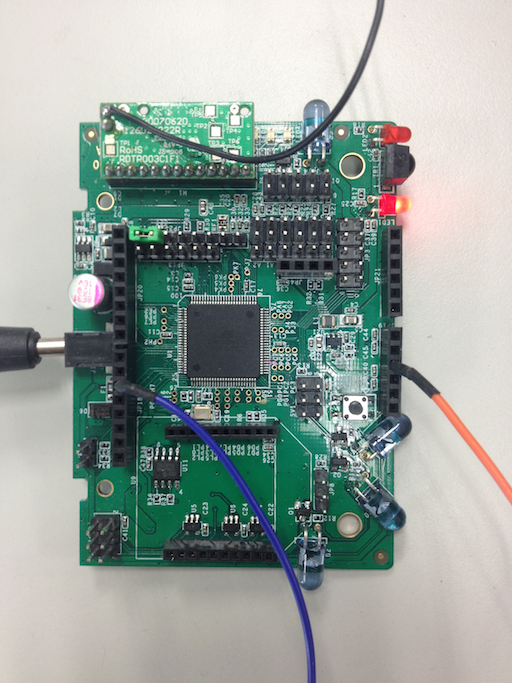
\includegraphics[width=\linewidth]{figures/wudevice}
\caption{An WuDevice equipped with ZWave radio on the top, and running
  a ATmega1280 8-bit microcontroller in the middle}
\label{fig:wudevice}
\end{figure}

\section{Experimental Setup}

%1(2)
%2(4)
%3(5)
%4(6)
%5(7)
%6(10)
%7(12)
%8(13)
%9(14)
%10(15)

\begin{table}
\centering
\caption{Node setup}
\label{tbl:setup}
  \begin{tabular}{|l|l|}
  \hline
  \textbf{Node Id} & \textbf{Equipped resources} \\
  \hline
  1 & Light Actuator \\
  \hline
  2 & Numeric Controller, Threshold, Light Sensor \\
  \hline
  3 & Light Actuator \\
  \hline
  4 & Light Actuator \\
  \hline
  5 & Light Actuator, Light Sensor \\
  \hline
  6 & Light Actuator \\
  \hline
  7 & Light Actuator \\
  \hline
  8 & Light Actuator \\
  \hline
  9 & Light Actuator \\
  \hline
  10 & Light Actuator \\
  \hline
  \end{tabular}
\end{table}

Ten WuDevices were deployed. Every WuDevice will be able to talk to each other
directly through ZWave adapter forming a fully connected network. Eight of them
were equipped with light actuators. Two of them have light sensors. Only one of
them has user input device (Numeric Controller), and Threshold. We simulate
a node failure by removing power supply of a WuDevice. The setup was shown in
table~\ref{tbl:setup}.

\section{Mapping Results}

The result of the mapping and the strips were shown in
table~\ref{tbl:mapping-result}. Each row represented each component in the
application, where strips were ordered from the left. Numeric Controller was
mapped to only node 1; Light sensor was mapped to node 2 and 5, where 2 hold the
active WuObjects when deployed; Light actuator was mapped to 9 nodes, and node
1 hold the active WuObject when deployed; Threshold was mapped to node 2.  The
result indicated that the only active nodes were 2, and 1 right after deployment.


\begin{table}
\centering
\caption{Strips}
\label{tbl:mapping-result}
  \begin{tabular}{|l|l|}
  \hline
  \textbf{Application Component} & \textbf{Mapped nodes (strip)} \\
  \hline
  Numeric Controller & 2 \\
  \hline
  Light Sensor & 2, 5 \\
  \hline
  Light Actuator & 1, 3, 4, 5, 6, 7, 8, 9, 10 \\
  \hline
  Threshold & 2 \\
  \hline
  \end{tabular}
\end{table}

%\section{Mapping method}

%Deployments with different strip ordering method, such as first-fit, last-fit,
%closest-fit, will be performed to compare their effects on system performance.

%As first-fit was introduced in eariler chapter at chapter~\ref{c:design}, the
%other methods that will be used in the experiment were introduced here.

%Last fit was exactly first fit but reversing the order at the end.
%Closest fit sorts the strips by the order of the histogram of number of unique
%capability a node has.


\section{Results}
\label{s:results}

The results for memory overhead by strips before failures were consistent as
shown in figure~\ref{fig:results-system-overhead-vs-network-size}, as each entry
in strip takes two bytes as one byte is used by node address defined in ZWave
protocol, the other byte was used for our internal WuObject identification
system to recognize wuobject on a node. The growth of the overhead is quadratic,
as shown in previous chapter that $O(m*n)$ when $m = n$. We have also observed
that none of the failovers were incorrect.

Table~\ref{tbl:results-memory-overhead-strip} listed the overhead of memory in
bytes used by each strip. Each entry in the strip consumes 2 bytes, one byte for
addressing and the other is for internal addressing for WuObjects. Strips for Light Actuator takes up 18 bytes because there are 9 nodes assigned as members.

The message overhead as related to the node as first failure is also shown in
figure~\ref{fig:results-message-overhead}. The size of message overhead was
measured by averaging 5 deployments of the number of messages sent or received,
including retries, by the detector during the recovery process multipled by the
maximum package size which was 32 bytes.

The detection time plus recovery time for different heartbeat period is plotted
in figure~\ref{fig:results-heartbeat-vs-detection-recovery-time}. Heartbeat
period is the interval between heartbeat messages a node sent to
another node for health monitoring. The detection time is the time from 
which a node failed to when the detector detects failure and initiated recovery
algorithm. It's not the same as recovery time, as recovery time is the time took
to recovery the network. The plot showed a linear relationship between heartbeat
period and total time to recovery from failure. Recovery time is relatively
constant in every deployment with the same network and strip size, therefore the
only deciding factor is heartbeat period. 

The figure~\ref{fig:results}
illustrates the average recovery time and message overhead over 5 deployments
for each node failure in Strip for Light Actuator as first failure in the
system. The first failure should on average takes the longest time and higher
message overhead compared to consequent failures. Therefore measuing the
performance for each node failure as first failure would give us how the system
would perform the worst overall. The results carried over even in different
strip orders for Light Actuator Strip since the ordering was just a matter of
permuting the results as shown in the results.

The recovery time for most nodes were averaging around 2500 milli-seconds; node
3 and node 6 were found out that their radios were a little defective (without
antenna) after the experiments therefore it took longer to complete the
recovery. It was clear that the results have shown were pretty consistent as
there were only a constant number of nodes that needed to contact to recovery
regardless of how many strips the node contained. The time it took was reasonable
given the small network. The above results have shown that the system
could sustain failures and reliably recover and maintain predictable performance
over a small network.



% TODO:Just pasted, need revision
Theoretically, deploying to a network with 10 nodes with a 5-component application, which was mostly
the maximum number of complexity a typical real-world application could have, can
operate reliably if each node could dedicate 100 bytes of memory to strips
(assuming one byte node addressing including the WuObject identification 
bit), and equipped with hardware
capable of handling approximately 20 messages for reconfiguration messages per
failure with a handful of room for retries. The requirements were reasonable since most embedded devices have at
least 4K of EEPROM to store strips, and have radios with throughputs of 40kbps.

The size of network was also feasible and the limiting factor is ZWave wireless
protocol since it only supports a network up to 232 nodes; nevertheless
a network of that size was pretty big for most real world deployments in areas
such as home automation which would require complex application logic and
service oriented architecture.

\begin{figure}[h!]
\centering
    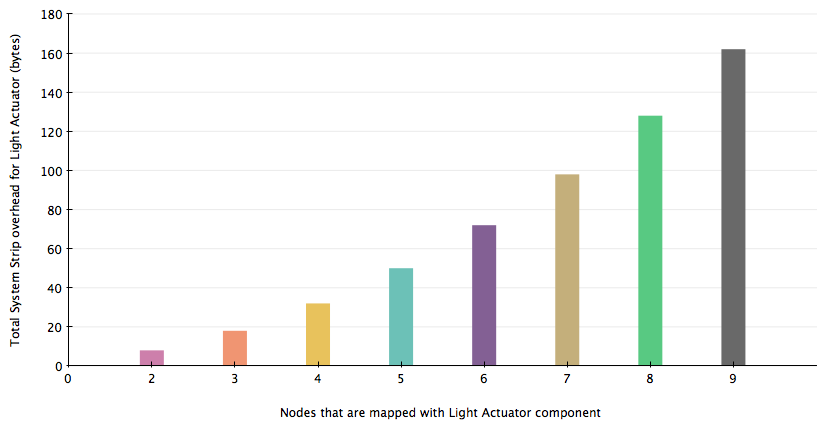
\includegraphics[width=\linewidth]{figures/results-system-overhead-vs-network-size}
\caption{Nodes taking Light Actuator component versus the overhead used by the
Light Actuator Strip}
\label{fig:results-system-overhead-vs-network-size}
\end{figure}

\begin{figure}[h!]
\centering
    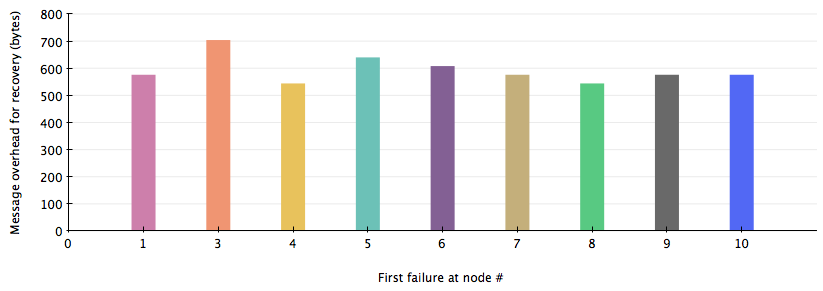
\includegraphics[width=\linewidth]{figures/results-message-overhead}
\caption{Message overhead used to recover for node as first failure}
\label{fig:results-message-overhead}
\end{figure}

\begin{figure}[h!]
\centering
    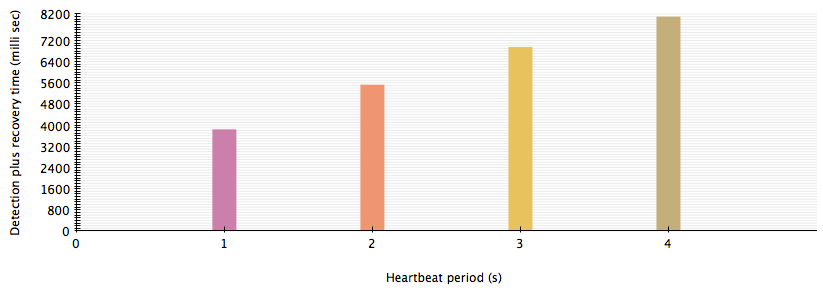
\includegraphics[width=\linewidth]{figures/results-heartbeat-vs-detection-recovery-time}
\caption{Detection plus recovery time in milli-seconds for heartbeat period in seconds}
\label{fig:results-heartbeat-vs-detection-recovery-time}
\end{figure}

\begin{figure}[h!]
\centering
    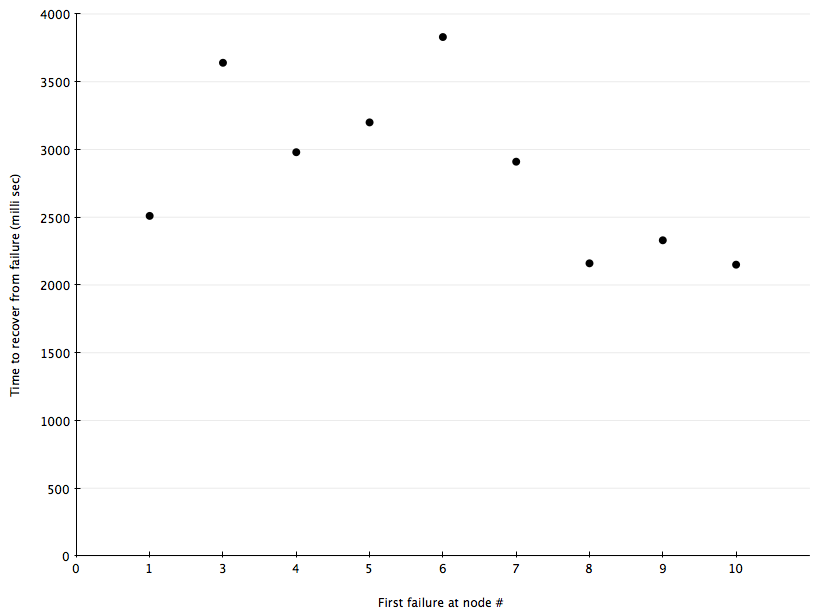
\includegraphics[width=\linewidth]{figures/results-average-recovery-time-plus-message-overhead}
\caption{Recovery time averaging over 5 deployments for each node failure as the first failure}
\label{fig:results}
\end{figure}

\begin{table}
\centering
\caption{Memory overhead of Strips in bytes}
\label{tbl:results-memory-overhead-strip}
  \begin{tabular}{|l|l|}
  \hline
  \textbf{Application Component Strip} & \textbf{Memory size (bytes)} \\
  \hline
  Numeric Controller & 2 \\
  \hline
  Light Sensor & 2 \\
  \hline
  Light Actuator & 18 \\
  \hline
  Threshold & 2 \\
  \hline
  \end{tabular}
\end{table}


\cleardoublepage
\singlespacing
\chapter{CONCLUSION}
\label{c:conclusion}
\doublespacing\nointerlineskip

%Previous chapters have described the work that has been done on WuKong platform.
%It is useful to reflect on what has been accomplished and place them in the
%broader context of the more general fault tolerance problem as well as the
%specific contributions of this work.

\section{Discussion}

This thesis proposed a novel algorithm to achieve
recovery from failures by combining heartbeat protocol, for failure detection,
with Strips, which are used to maintain and track service redundancy.

We have presented a fault tolerance system able to provide failover for failed
services in service-oriented WSNs that comply with user policy requirements. We
have also described strip, a redundancy abstraction for service peers along with
distributed algorithms to synchronize strip views among members and
reconfigurate the network for the new structure to recover from node failure.
The system allows user intervention through means of user policy, which could
directly influence underlying system configurations and structure.

The developed methods add new and useful solutions to build a fault tolerant
system that could be reasoned easily and with a performance as expected on
average. This method makes an extension to other methods in terms of
completeness and complexity. It serves as a quick and easy solution
to provide practical fault tolerance for WuKong applications.

% TODO: summarize the results of the experiments here, etc
% e.g. The solutions developed for WuKong system performs very consistently, as
% the recovery time is always under two secs on average with a handful of
% sensors. However, occationally heartbeats could report erroneous failures and
% result in a quick false recovery, and left the partitioned nodes behind, but
% the system as a whole still function properly.

The experimental results have shown to be consistent and stable among first
failures in different rank of members in strip around 2.5 secs. The failover
have been successful in all deployments. It is also shown that the performance
degraded quickly when the hardware or the wireless communication quality
degraded. Therefore it is important that the network setup is as optimized as
possible. 

\section{Future Work}

% Probably move it to future work? Probably don't do it.
%Of course there are a lot of room for improvements. For example, if we want to
%go beyond this limitation of 232 nodes by Zwave, one of the ways we could do is
%to build another zwave network and have a routing agent to route messages
%between networks. And we would also want to handle network partitions. One of
%the possible research directions is to merge the partitions back to one if they
%come back together, or by using some arbitrary flags to indicate primary
%components in the network to eliminate redundant commanding network components.
%Nonetheless, it is also an opportunity to look into multi-hop networks since
%heartbeats protocols are designed with single-hop network in mind, whether we
%could change the protocol to handle multi-hop is also a big challenge a future
%research could take on.


We have shown a design for a reconfigurable fault tolerant system for WuKong.
Strips makes it really easy to describe a component system with redundancy for
heterogeneous services and devices. Nevertheless, there is still room for
improvements. This section will address some directions future research can take.

WuKong Fault Tolerance System did not consider for network partition. Network
partition occurs when a network of nodes got partitioned into two subnetworks where
none can detect each other for a period of time. One of the possible direction
is to create a more sophisticated failure model that could handle network partition.
In this thesis we assume failstop model where nodes, once dead, will not come
back. Therefore when network partition occurs, each part of the network would
not be able to recognize each other and would cause conflicts and confusions.

Our current heartbeat protocol is distributed and easy to construct, but it is
not shown to work under networks where messages are sent in multiple hops, since
the algorithm used to produce where each node should be sending heartbeat
messages does not consider the topology of the network. Heartbeat is sensitive
on latency, so if a heartbeat message was not received within tolerance period,
a failure event could occur and the node is suspected of failure and will
never come back. If the node is still alive, it would be treated as if it is
dead. And that will creates an artificial network isolation where a few nodes
are excluded from the network before of latency.

Current system can only allow the detector to handle one failure at a time. It
would be a desirable future research direction to investigate handling
consecutive node failures. One possible way is by storing ahead multiple nodes'
strips and heartbeat protocol data, such that when consecutive nodes failure
occurred the detector would be able to recover those services it backed up.
However there is a tradeoff on the memory a node could store and the number of
consecutive node failures a network could handle.

\begin{comment}
Niels suggested that I show that I am aware of such issue with determining
optimality for deployment which is not clear for WuKong yet, there are many
ways or metrics to optimize for, all I can do in this work is to identify some
tradeoffs certain deployment for fault tolerance could influence the system
with certain metrics.

Limits will be hard to define here
Niels:about the tradeoffs in determining the deployment from your fault
tolerance perspective
Penn:Remember what the prof told me, about policy, first fit, last fit, etc
\end{comment}

The optimization problem for application deployment is also an important element
in this system. This thesis didn't consider finding a optimal deployment for the
level of redundancy specified in the user policy. The problem of deploying
a specific distributed system onto a network structure typically consists of
mapping the components of the system onto the hosts of the network. The mapping
is subject to constraints. The constraints could be whether a node supports
certain service to host certain components, and how much communication overhead
would induce from the assignment to maintain consistency for the strips, and
from the perspective of WuKong, some components need to seaparate from other
components to achieve fault tolerance, and some needs to place together to
function properly.  Determining such an optimal deployment is a combinatorial
optimization problem, and combinatorial optimization problems generally
extremely challenging computationally. It is difficult to predict what will and
what will not work.  It is unlikely that a single approach will be effective on
all problems or instances of the same problems. As we also want the system to
come up with a solution within a time limit. So finding a good balance between
the quality of a solution of the time it takes to come up with a good enough
solution is critical.


\backmatter

\addcontentsline{toc}{chapter}{\bibname}
\bibliographystyle{ieeetr}
%\bibliographystyle{apalike}

% input your reference here
%\bibliography{thesis}
\bibliography{/Users/penn/Documents/Bibtex/Thesis.bib}

\appendix

\end{document}
